\documentclass{purdue-slide}

% For filler text:
\usepackage[base]{babel}
\usepackage{lipsum}

% \renewcommand{\titlelogo}{logo/cs-rev.svg}
% \renewcommand{\slidelogo}{logo/cs.svg}
% For non-CS Purdue logo use the lines below:
\renewcommand{\titlelogo}{logo/ece-rev.svg}
\renewcommand{\slidelogo}{logo/ece.svg}
% You can also request a logo from https://marcom.purdue.edu/toolbox/logos/

\title{Functional Programming \& Category Theory}
\subtitle{An Informal Introduction}
\author{Aadi Rave}
\institute{Purdue University}
\date{\today}

\begin{document}

\begin{titleframe}{}
    \maketitle
\end{titleframe}

\section{What is Functional Programming?}

\begin{titleframe}{A Quick Intro to Functional Programming}
Function composition, higher-order functions \& immutability
\end{titleframe}

\begin{frame}{The Commandments of FP}
    \begin{itemize}
        \item Thou shalt use \textbf{pure functions}
        \item Thou shalt avoid \textbf{mutable state}
        \item Thou shalt embrace \textbf{first-class functions}
        \item Thou shalt use \textbf{higher-order functions}
        \item Thou shalt favor \textbf{function composition}
        \item Thou shalt use \textbf{recursion}
        \item Thou shalt swear allegiance to \textbf{monads}
        \item Thou shalt keep code \textbf{declarative}
    \end{itemize}
\end{frame}

\begin{frame}{The Important Stuff}
    \begin{itemize}
        \item \textbf{Immutability} Once data is created, it should not be modified. 
        \item \textbf{Pure Functions} Do not depend on program state, and do not modify program state.
        \item \textbf{First-Class Functions} Treat functions as values -- return them, pass them as arguments, assign them to variables
        \item \textbf{Higher-Order Functions} Compose simple functions to do complex things
    \end{itemize}
\end{frame}

\begin{frame}{A Quick Demo of Function Composition}
    Consider the simple problem of taking the sum of squares of even numbers in a list. Let's compare the C and OCaml ways of solving the problem.
\end{frame}

\section{What is Category Theory?}

\begin{titleframe}{An Informal Intro to Category Theory}
Objects, Morphisms, Functors \& Monads
\end{titleframe}

\begin{frame}{What is a category?}
    Think of category theory as the mathematics of \textbf{structures} and their \textbf{relations}. A category consists of \begin{itemize}
        \item \textbf{objects}
        \item \textbf{morphisms}
    \end{itemize}
\end{frame}

\begin{frame}{Properties of Categories}
    \begin{itemize}
        \item \textbf{Composition} $$\forall f: A \rightarrow B, g: B \rightarrow C, \exists g \cdot f: A \rightarrow C$$
        \item \textbf{Associativity} $$(h \cdot g) \cdot f = h \cdot (g \cdot f)$$
        \item \textbf{Identity} $$\exists id_{A}: A \rightarrow A, id_{B}: B \rightarrow B \ni f \cdot id_{A} = f, id_{B} \cdot f = f, \forall f: A \rightarrow B$$
    \end{itemize}
\end{frame}

\begin{frame}{Partial Ordering as a Category}
    Partial Ordering has three properties: \begin{itemize}
        \item \textbf{Reflexivity} $$a \leq a$$
        \item \textbf{Antisymmetry} $$a \leq b, b \leq a \implies a = b$$
        \item \textbf{Transitivity} $$a \leq b, b \leq c \implies a \leq c$$
    \end{itemize}

    Think of the properties of a category: composition, associativity, and identity. Let's see how partial ordering fulfils each of them.
\end{frame}

\begin{frame}{Functors}
    A \textbf{functor} is a morphism between categories, ie. a functor $T: A \rightarrow B$ maps each object of category $A$ to an object in category $B$ and each morphism in category $A$ to a morphism in category $B$. 
\end{frame}

\begin{frame}{Monads}
    A \textbf{monad} is like a pattern that helps you manipulate data types, and actions, while dealing with their side effects elegantly. 

   \par \medskip A monad has three parts: \begin{itemize}
        \item A functor $T$ to add extra context to a value
        \item A unit $\eta$ which takes a value and wraps it in $T$
        \item A multiplication operator $\mu$ to unwrap a value from the context
    \end{itemize}

    \par \medskip In the real world, we change what our components do and what our functor is, depending on requirements. Let's look at Option types using a simple Python implementation.
\end{frame}

\begin{frame}{Bonus: Kliesli Categories}
    What if you want to compose monads? If you apply the $\eta$ function on an object $A$ twice, we get $M(M(A))$, which we can't deal with using $\mu$! The solution? A \textbf{Kliesli Category}. Intuitively, we use these to "flatten" objects from $M(M(A)) \rightarrow M(A)$, allowing us to compose monads! Let's go back to our previous example and see it implemented in Python.
\end{frame}

\section{Why}

\begin{titleframe}{Monads Everywhere}
Every problem in programming can be solved using abstraction -- except using too much abstraction. With great power comes great responsiblity!
\end{titleframe}

\begin{frame}{Applications}
    \begin{itemize}
        \item Error Handling
        \item Concurrency
        \item List comprehension
    \end{itemize}
\end{frame}

\begin{frame}{Error Handling with Monads}
    Here's some error checked OCaml code to extract an integer from a string:
    \begin{figure}
        \centering
        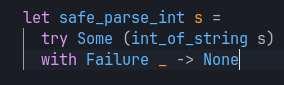
\includegraphics[width=0.5\linewidth]{image.png}
    \end{figure}

    \par \medskip Compare this to error checking a C function like \texttt{strtol}! \par \medskip Languages like \textbf{Rust} and \textbf{Scala} have adopted the monadic way of handling errors. Pointers in newer languages like \textbf{Zig} can be made optional using monadic logic behind the scenes.
\end{frame}

\section{Further Reading}

\begin{titleframe}{Further Reading}
\end{titleframe}

\begin{frame}{Textbooks}
    Ordered from least formal to most formal, some resources to check out are: \begin{itemize}
    \item \href{https://bartoszmilewski.com/2014/10/28/category-theory-for-programmers-the-preface/}{Category Theory for Programmers (B. Milewski)}
    \item \href{https://books.google.co.in/books/about/Basic_Category_Theory_for_Computer_Scien.html?id=ezdeaHfpYPwC&redir_esc=y}{Basic Category Theory for Computer Scientists (B. Pierce)}
    \item \href{https://www.google.com/books/edition/Algebra_Chapter_0/deWkZWYbyHQC?hl=en&gbpv=1&dq=algebra:+chapter+zero&printsec=frontcover}{Algebra: Chapter Zero (P. Aluffi)}
    \item \href{https://github.com/geelon/type-theory/blob/master/awodey-category-theory.pdf}{Category Theory (S. Awodey)}
\end{itemize}

\end{frame}
\end{document}